\documentclass[10 pt, conference]{ieeeconf}

\pdfminorversion=4

\usepackage{mathrsfs}
\usepackage{amssymb}
\usepackage{cite}


\usepackage{mathrsfs}
\usepackage{amssymb}
\usepackage{amsmath}
\usepackage{cite}
\usepackage{graphicx}
\usepackage{color}
\usepackage{float}
\usepackage{multicol}
\usepackage{multirow}
\usepackage[bb=boondox]{mathalfa}	% allows for double-struck 1

\newcommand{\proofbox}{\hfill\mbox{$\blacksquare$}}
\def\qed{ \rule{.1in}{.1in}}
\def\eq#1{\begin{equation}#1\end{equation}}
\def\eqa#1{\begin{eqnarray}#1\end{eqnarray}}
\def\eqan#1{\begin{eqnarray*}#1\end{eqnarray*}}
\newcommand{\ga}{\alpha}
\newcommand{\sk}{\vspace{1ex}}
\newcommand{\rank}{{\rm rank\;}}
\newcommand{\lcm}{{\rm lcm}}
\newcommand{\argmin}{{\rm argmin\;}}
\newcommand{\image}{{\rm image\ } }
\newtheorem{thm}{Theorem}%[section]
%%%%%%%%%%%%%%%%%%%%%%%%%%%%%%%%%%%%%%%%%%%%%%%%%%%%%% Main Body%%%%%%%%%%%%%%%%%%



\IEEEoverridecommandlockouts
\overrideIEEEmargins


\title{\LARGE \bf Adaptive Cyclic Pursuit for robust decentralized circular formations with non-holonomic agents
}


\author{ Enrique Babio %\quad  Shaoshuai Mou
	\thanks{
		%S. Mou is with the School of Aeronautics and Astronautics, Purdue University, West Lafayette, IN 47906. {\small \tt{mous@purdue.edu}}; 
		E. Babio is currently pursuing a MSc in Aeronautics and Astronautics in Purdue University. {\small \tt{ebabiofe@purdue.edu}}.}
}


\begin{document}



\maketitle
\thispagestyle{empty}
\pagestyle{empty}


%%%%%%%%%%%%%%%%%%%%%%%%%%%%%%%%%%%%%%%%%%%%%%%%%%%%%%%%%%%%%%%%%%%%%%%%%%%%%%%
	\begin{abstract}
	An adaptive control law for achieving circular formations is proposed for non-holonomic agents (steered particles). The control law relies on the Cyclic Pursuit algorithm where every agent $i$ pursues agent $\mod(i+1,n)$ with some offset bearing. If the pursuing pattern follows a ring directed graph and some global conditions on the bearing offsets are met  a circular formation can be achieved .Typically, this bearing offsets have been assigned a priori to meet this circle convergence condition. This work proposes an adaptive variation of the control law that achieves convergence with no knowledge a priori knowledge of the bearing offsets and relying only on local measurements. As such, the algorithm is robust to changes in the network and only implies that the agents are connected forming a ring directed graph. Following this new approach control laws for the control of the radius and for achieving spacing are proposed that work under the new adaptive control. Partial proofs for convergence are provided.
\end{abstract}

\section{Introduction}
Circular formations arise in natural behaviors in the animal kingdom: schools of fish \cite{parrish2002self} or groups of vultures stalking a prey exhibit this behavior according \cite{cone1962thermal}. From an aerospace point of view the vulture behavior is pretty remarkable since they use thermals to stay airborne with little or no effort. This behavior is also interesting for engineering applications. Using thermals to minimize fuel consumption for loitering aircraft is an interesting application \cite{akos2010thermal}. But we can think of other applications, such as UAVs being used for observation as proposed by Ma and Hovakimyan in \cite{ma2013cooperative}. 

In the simplest Cyclic Pursuit setup, each agent $i$ follows the immediately preceding agent denoted as $\mod(i+1,n)$ so the global connectivity graph is a strongly connected ring directed graph. In this condition all agents will achieve consensus simultaneously for random initial conditions as shown by Richardson \cite{richardson2001nonmutual}.

If instead of trying to capture the preceding agent we try to maintain a constant bearing with respect to it then circular formations can be achieved, which is the topic interest here. Some conditions for cyclic formations can be found are stated by Tabuada \cite{tabuada2001cylic}. The general solution for this strategy are spirals converging or diverging from the center and the circular formation is just the transition between them depending on some global conditions. Marshall and Francis \cite{marshall2004formations}  prove the single integrator to be stable using circulant matrices with is a single eigenvalue at the origin and all others are stable, a recurring result for distributed algorithms. 

Ramirez et al \cite{ramirez2010distributed} have extended the algorithm to control the radius of the formation and double integrators. The control of the radius relies on controlling the distance to the previous agent, if we know the relationship between the formation radius and the distance to the previous agent then the converging or diverging behaviors of the spiral can be excited. Some other notable work on single integrator dynamics is that of Zhao \cite{zhao2014distributed} where formations can be achieved using bearing-only measurements which is a new approach to the topic.

However, by choosing the non-holonomic steered particle our model is more restrictive and with a greater interest to the aerospace field. Typically, maneuverability on the longitudinal axis is restricted for fixed-wing aircraft where the range of accelerations is usually quite small and not all velocities are possible. 

The Cyclic Pursuit algorithm for non-holonomic particles were first introduced by Justh and Krishnaprasad in \cite{justh2002simple}, \cite{justh2003steering}. Marshall and Francis \cite{marshall2004formations} proved that the non-holonomic evenly-spaced  formation is locally stable by linearizing the formation about the equilibrium invariant set. Global conditions for convergence to the circle are given by Galloway, Justh and Krishnaprasad in a later work\cite{galloway2013symmetry} by the defining the dynamics of the Cyclic Pursuit manifold. They show that any initial state will converge to this manifold and then they study the behavior of the formation in terms of some global conditions. The global conditions for convergence to a circle are found irrespective of the spacing between agents and how those are related to the converging and diverging behavior.

Advancements on the robustness have been made by Fathian et al \cite{fathian2016distributed}. Their approach is based on defining some target position of the agent as a function of the preceding and trailing agents. An extra measurement is included but the algorithm becomes robust to changes in the the behavior of the network. Morbidi et al \cite{morbidi2010maintaining} have studied the effect of communication and sensor range in achieving the formation by focusing on the initial conditions and the transients before the formation is achieved. Sharma et al \cite{sharma2012cylic} have introduced a collision avoidance into the double integrator problem by means of a gravity-like repulsion force, and with agent with a modified control law that prevents the formation from diverging. Daingade et al \cite{daingage2016failsafe} have addressed the convergence with no cordination but relying on bearing measurements to all the agents in the network which is a somehow similar approach.

All these algorithms rely on local coordination, but still use some global information or coordination. A ring directed graph (di-graph) is needed and the conditions for convergence are given in terms of global characteristic that have to previously agreed. Pavone and Frazzoli \cite{pavone2007decentralized} define a strategy to achieve a ring di-graph by exploiting the fact that a circular formation will have all its agents in the boundaries of a convex set. An agent can find if it is in the convex set boundary of the formation and in the negative case move there. Once all agents are in the border they can follow the preceding agent that in this case will be in an extrema of the observed bearings to all other agents.

As of now we know that a circle can be achieved if some global conditions are met. But no work has addressed the fact the challenge of arriving to a circular formation with no global coordination at all for any possible network. Here lies the innovation of this work, we propose an adaptive local coordination control law that ensures the global conditions are met without any previous coordination or information. To the best knowledge of the authors, this is the first approach to achieve this feature. This is our main result, and it is proved to converge to a circle. These circular formations have no predetermined radius, or spacing. Two strategies for achieving a desired radius and spacing are proposed. The main result and the two proposed strategies are shown to converge to controlled circular formations in simulations for several cases including time-varying networks.

This text is organized as follows. Section 1 has defined the motivation for the problem. Section 2 introduces the Cyclic Pursuit algorithm as defined in \cite{galloway2013symmetry}, conditions for convergence and some issues that may arise. Section 3 introduces the main contribution, the adaptive control law, defining its assumptions, to allow for circular convergence with no global information. Section 4 introduces the complimentary results, control laws for the control of the radius and the spacing og the formation discussing their implications on measurements. Section 5 illustrates the results with simulation showing some issues of the initial algorithm and shows convergence for the adaptive algorithm under a variety of conditions. Section 6 provides some conclusions and discusses further work. Partial proofs for the convergence of the adaptive algorithm can be found in Annex A.
\section{Problem Formulation}

Cyclic pursuit is a distributed algorithm for achieving circular formations. In particular, we assume each agent knows its own state and that of the preceding agent in the formation. In order to achieve a circle the network must be strongly connected and therefore the corresponding graph for the network is the stated ring di-graph. The algorithm is based on continuous time dynamics and controls.

In order to describe the formation achieved we start by describing the dynamics of the system. Each individual agent is described as a non-holonomic particle with a common constant velocity that can be steered using the input. Its dynamics with respect to an some reference frame are
\begin{align}
\dot{x}_i &= v \cos \psi_i \\
\dot{y}_i &= v \sin \psi_i \\
\dot{\psi}_i &= u_i  
\end{align}

$\vec{r}_i=(x_i,y_i)$ represent the Cartesian coordinates on the euclidean plane for the position of agent $i$. $v$ is a constant velocity, common for all agents, and $\psi_i$ the heading of the velocity which can be modified by means of the control input $u_i$.

Each agent $i$ knows its own state in a local reference frame. It is also able to measure the relative position of the preceding agent $j= \textrm{mod}(i+1,n)$ and heading of its velocity with respect to some local reference frame. All the information about the agent $j$ can be achieved without any communication between the agents by relative position measurements. This feature is highly desirable and we will try to preserve by all means.

The relative position vector $\vec{r}_{ij} = \vec{r}_j - \vec{r}_i$ is expressed in a local coordinate frame by its module $\rho_{ij}$ and relative its argument $\kappa_{ij}$ with respect to the velocity heading $\psi_i$. The relative argument between the heading of the velocity preceding agent $j$ $\psi_j$ and the $\vec{r}_{ij}$ vector is defined as $\theta_{ji}$. These two parameters are determined by the relative position measurement.
\begin{figure}[h]
	\centering
	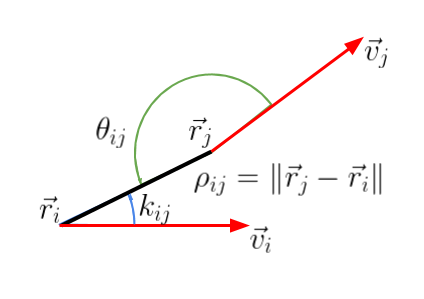
\includegraphics[height=1.7in]{Attachments/Geometry.png}
	\caption{Description of the geometry between agent $i$ and $j$.}
	\label{fig:Geometry}
\end{figure}

Cyclic pursuit attempts to keep this relative bearing $k_{ij}$ constant and equal to the reference $\alpha_i^*$. $^*$ all along this report will mean that some value is constant and predetermined. $\mu$ is a positive gain that controls the control action proportional to the difference between the actual relative bearing $\kappa_{ij}$ and the reference $\alpha_i$. The control law used to achieve this is given in \cite{galloway2013symmetry}
\begin{equation}
  u_i = \mu  \sin(\kappa_{ij} -\alpha_i^*) + \frac{1}{\rho_{ij}} ( \sin \kappa_{ij} + \sin \theta_{ji})
\end{equation}

The control law is the addition of two terms. The first term is a proportional-like term that intends to make the actual relative bearing $\kappa_{ij}$ converge to the desired relative bearing $\alpha_i^*$. The second term attempts to compensate for the angular motion between the two agents. This is done by computing the lateral velocity between $i$ and $j$ as the projection of the velocities of $i$ and $j$ along the relative position vector. This lateral velocity is converted into angular rate using the inter-agent distance $\rho_{ij}$.

This control law is shown to guarantee to converge to some formation in \cite{galloway2013symmetry} where the convergence is shown by showing the asymptotic stability of the network to some formation manifold. 
If all the agents have an equal constant velocity the shape of the formation is determined by $\alpha^* = [\alpha_1^* \quad \alpha_2^* \quad \ldots \quad \alpha_n^*]^T$ for agents $\ i\in\{1,2, \ldots, n\}$ as shown in \cite{galloway2013symmetry}. Furthermore, it shown that to achieve circular formations it is necessary that all $\alpha_i^*$ have the same sign. Without loss of generality, we consider only positive $\alpha_i^*$ from here on. 

Under those conditions, the same reference states Cylic Pursuit will converge into a converging/diverging spiral, and under certain conditions it will converge into a circle. The condition for the circular formation with no overlap is
\begin{equation}
  \alpha^{*T} \mathbb{1} = \pi
\end{equation}

The simplest formation satisfying the previous conditions achieves the regular n-sided polygon by using $\alpha_i = \pi / n$. We can see that under this conditions, and for $n=4$ the circular formation in the introduction is achieved.
\begin{figure}[h]
	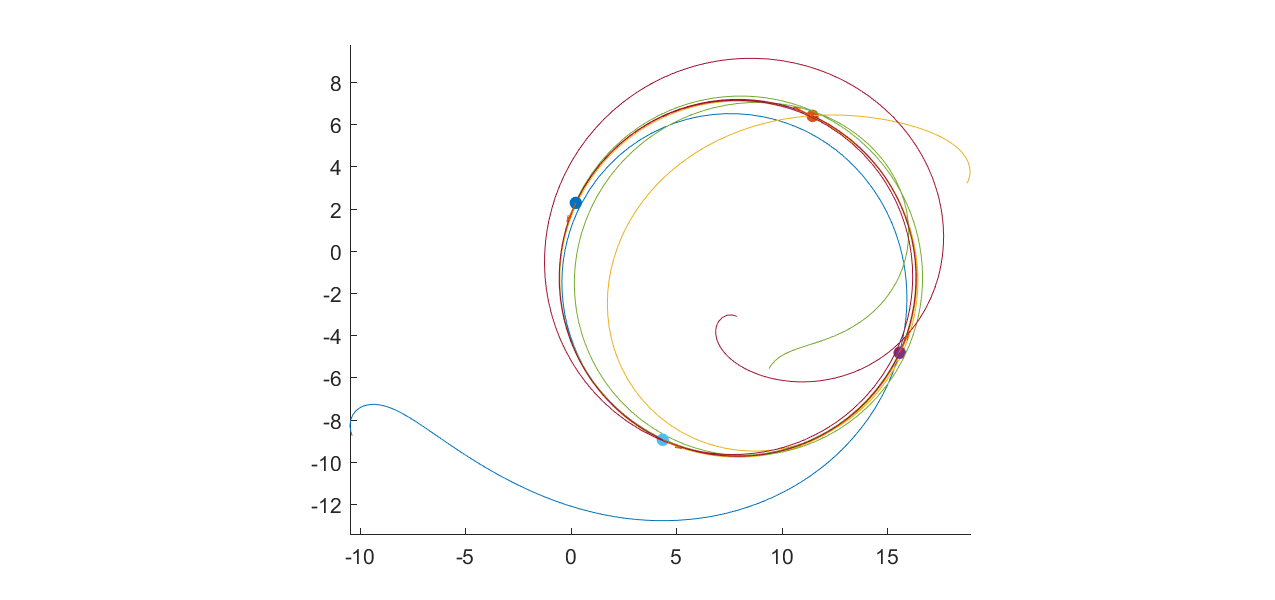
\includegraphics[width=\linewidth]{Attachments/Figure21.png}
	\caption{Cyclic Pursuit convergence to a circle.}
	\label{fig:CircleConvergence}
\end{figure}

Besides, the conditions for convergence (divergence) from the center are $\alpha^{*T} \mathbb{1} > \pi ( < \pi)$, then the spiral will diverge (converge). This fact will be leveraged in the upcoming sections.

While this algorithm is interesting from a theoretical point of view it has two main disadvantages that prevent its application

\paragraph{Radius stability}
The stability of the algorithm relies completely on angular criteria on the circle. These criteria are independent of the radius implying there is no control on the radius and size of the formation nor stability under perturbations.

Another issue is the difficulty to predict the parameters of the final formation given the initial conditions. No prediction on the size of the formation (even if no perturbations are present) can be obtained by inspection of the initial conditions.

\paragraph{Network robustness}
The convergence of the algorithm to a circle relies on achieving the $\alpha^{*T} \mathbb{1} = \pi$ criterion. This implies the need of coordination and that if an agent leaves or joins the formation will no longer work. Typically, adding a new agent will increase the sum of the elements of $\alpha^{*T} \mathbb{1}$ and removing an agent will reduce it. The algorithm is not robust from a network variation point of view.

A solution to the radius stability is provided in \cite{ramirez2010distributed}. This solution however, is dependent on the $\alpha^{*T} \mathbb{1} = \pi$ condition and therefore is not considered to be robust to changes in the network. In order to provide a better understanding of the solution we will first give a more insightful description of the two issues that will be addressed in this project.




\section{Main Results}

This section introduces the approach used to solve the two issues we have identified: radius stability and network robustness. This is done by defining a $\alpha_i$ not as a reference, but as an state that is modified to control the shape of the formation by some adaptive control laws. While the goal of Cyclic Pursuit is to achieve a formation, these control laws modify the shape of the formation.

In order to prevent the adaptive shape control laws from interfering with Cyclic Pursuit and therefore not achieving any formation at all, the only assumption is introduced

\textbf{Assumption 1}. The effect of the adaptive shape control law is negligible outside the formation manifold. They are designed accounting for the dynamics of the formation in the manifold and only there they are guaranteed to converge.

The adaptive shape control law is composed by adding three terms. Each of these terms are independent and have different goals. The goals are circularizing the formation, achieving uniform spacing, and converging to a predefined radius. Each one of them will output a specific adaption rate that for each agent $i$ that we will denote with $\dot{\alpha}_{ci}, \dot{\alpha}_{si}, \dot{\alpha}_{ri}$ respectively. Each of them is modulated with a gain which will be similar to all agents. Therefore the final adaption rate can be computed as
\begin{equation}
\label{adaptiveLaw}
  \dot{\alpha}_i = \mu_c \dot{\alpha}_{ci} + \mu_s \dot{\alpha}_{si} + \mu_r \dot{\alpha}_{ri}
\end{equation}

We will now describe how to handle the assumption we have introduced from a practical point of view and the expression for the terms of the adaptive control shape control law.

\subsection{Implications of Assumption 1}
The stated assumption has two implications on the practical implementation of the algorithm.

\begin{enumerate}
	\item A switching strategy that enables/disables the adaptive shape control law should be available so that while the network is converging to some formation the control adaptive shape control laws are disabled. This switch should be designed taking into account only information that was previously available for each agent so it doesn't affect the distributed nature of the control (i.e measurements of previous agent only).
	
	\item A more restrictive switching strategy, less tolerant about errors, will be more robust against undesired changes in $\alpha_i$, but will take more time to converge. Furthermore, using only locally available information means formation errors happening in other parts of network may be unnoticed. Conversely, a more tolerant strategy should be coupled with smaller adaption rate to ensure that the transients due to adaption do not affect the convergence of the adaptive control laws themselves. 
\end{enumerate}

A possible switch is proposed here, and will be used in the simulations. However for the purpose of proving the validity of the control laws it is assumed to satisfy Assumption 1.

Ideally the value of the switch should be 0 if a formation has not been achieved and 1 if the formation is achieved. If we choose a smooth switch and we define it in terms of some formation error, then it should be 1 at 0 error and 0 as the error grows. A possible candidate for this function is a gaussian-like function with a maximum at 1. A possible measure of error is the relative bearing error. The resulting detector $\nu_{i}$ would be
\begin{gather}
\label{switch}
\nu_{i} = \exp(-\epsilon \sin^2(\kappa_{ij} -\alpha_i))
\end{gather}

Where $\epsilon$ would be some positive value that defines the tolerance of the switch. The smaller it is the more tolerant the switch.

\subsection{Circularization of the formation}
As stated before, not every relative bearing $\alpha$ will result in a stable circular motion, however it is guaranteed that all formations will converge to a spiral. A spiraling formation can be easily detected by measuring the rate of change of the distance $\dot{\rho}_{ij}$ between the agent $i$ and the preceding $j$.

We know that any $\alpha$ such that $\alpha^T \mathbb{1} = \pi$ will result in a circular formation. Also if $\alpha^T \mathbb{1} > \pi$ the formation will spiral outwards and vice versa. So an intuitive control law would be to decrease $\alpha_i$ if the inter-agent increases in order to decrease the global $\alpha^T \mathbb{1}$. In order to achieve convergence the change in $\alpha_i$ should at least follow the dynamics of a first-order integrator, so the expression we should use is
\begin{equation}
\label{circle}
  \dot{\alpha}_{ci} = - \dot{\rho}_{ij}
\end{equation}


The rate of change of the distance using can be estimated using only position and heading of velocity measurements. For that, we project the velocity of both the agent $i$ and the preceding agent $j$ on the relative position vector
\begin{gather}
  \dot{\rho}_{ij} = \frac{1}{\rho_{ij}} (\vec{v_j} \vec{r_{ij}} - \vec{v_i} \vec{r_{ij}}) = v (\cos(\kappa_{ij}) - \cos(\theta_{ji}))
\end{gather}

The circularization shape control law looks like
\begin{equation}
  \dot{\alpha}_{ci} = -\dot{\rho}_{ij} =  v (\cos(\kappa_{ij}) + \cos(\theta_{ji}))
\end{equation}



\subsection{Assembly of the adaptive control law}
In the formulation of the adaptive shape control law the applied adaption rate was defined. After defining the terms of the adaptive control law and the switch we recall the previous formulation introducing the switching gain term defined (\ref{switch}) and with the term defined in (\ref{circle})
\begin{equation}
\label{shapeControlLaw}
\dot{\alpha}_i = \nu_i \mu_c \dot{\alpha}_{ci}
\end{equation}

Values for $\nu_i(\epsilon)$ and $\mu_c$ should be chosen so that Assumption 1 is guaranteed. Typically, a big $\epsilon$ and a small $\mu_c$ will offer a more robust controlled converge but slower.

\textbf{Theorem 1}. Given a switching strategy and $\mu_c>0, \mu_s, \mu_r$ gains that guarantee that Assumption 1 is satisfied, the circularization control law in (\ref{shapeControlLaw}) makes the circular formation manifold globally asymptotically stable. Any initial state ($[\vec{x}, \vec{y}, \vec{\psi}, \vec{\alpha}]$) of the network converges to a circle without any coordination between agents.

A proof for Theorem 1 can be found in the Annex A

\section{Complementary results}
In this section we propose two extra control laws for controling the radius of the formation and 

\subsection{Equally spaced formation}
The procedure described in the previous section achieves a circular formation but there is no constraint on the spacing between any agents. Since each agent only uses the distance with respect to the preceding agent there is no way to obtain equally spaced formations. This can be solved by incorporating information about the pursuing agent $h = \textrm{mod}(i-1,n)$. The intuition is that the distance to both the preceding and pursuing agent should be the same. In order to increase the distance with respect to the preceding agent the $\alpha_i$ must increase, so the preceding agent is seen with a greater angle within the circle. 

Finally, it is non-dimensionalized with respect to some distance $\rho^*$, typically the desired radius $\rho^*=r^*$, to prevent different behavior for different radii of the circle.
\begin{equation}
\label{spacing}
\dot{\alpha}_{si}= \mu_2 \frac{\rho_{ih} - \rho_{ij}}{\rho^*}
\end{equation}

Adding this term to the previous term, we can achieve an equally spaced formation.

\subsection{Formation radius control}
The concept of formation radius only makes sense if a circular formation is achieved. If the formation achieved is a spiral there will be no radius. The formation shape control law to achieve a circle was described in the previous section, here we will assume that a circular formations has already been achieved to derive how to modify the radius of a circular formation.

In order to control the radius of the formation it is necessary first to have an estimate of the actual radius. Since we assume that a circular formation is achieved the dynamics of the particle $i$ satisfy
\begin{equation}
r_i \dot{\psi}_i = v
\end{equation}

Since $v$ is constant and known, an estimate $\hat{r_i}$ for $r_i$ is
\begin{equation}
\hat{r}_i = \frac{v}{\dot{\psi}_i}  = \frac{v}{u_i}
\end{equation}

Intuitively, if the reference radius $r^*$ is bigger than the estimated radius we will want to increase the radius, in a circular motion this can be achieved by decreasing the angular rate $\dot{\psi}_i$. 
\begin{equation}
\hat{r_i} - r^* = - \left( \frac{v}{u_i} - r^* \right)
\end{equation}

However, this approach would interfere with the adaptive circular motion control law so that it modifies the $\alpha$ due to the radial velocity. To avoid that, we will also use this term as a driver for $\dot{\alpha}$ decreasing $\alpha$ when we want to increase the radius of the formation. Under no damping, this would lead to oscillations around the desired radius $r^*$ since this behavior is described by a second order system. However, we know that our previously designed $\dot{\alpha}_{ci}$ acts precisely as a term damping the change in the radius, as long as both terms are active the radius control will be stable.

This control law is not well defined, since the control variable is in the denominator. A better conditioned alternative is to use the angular rate reference $\psi^*$ that is determined by the desired radius and velocity 
\begin{equation}
\psi_i - \psi^* = u_i - \frac{v}{r^*}
\end{equation}

Once again, this control law is derived assuming the formation has been achieved. This means that it will be useful to use the same switch as in the case of the circularization law. Even though this control law is easier to understand if the formation is circling, it may be useful to enable it even if the formations is still spiraling. E.g. is the radius is too big and the formation is collapsing it is useful to preserve this behavior until the desired radius is achieved. The final adaption rate for the radius is

\subsection{Assembly of the adaptive control law}
In the formulation of the adaptive shape control law the applied adaption rate was defined. After defining the terms of the adaptive control law and the switch we recall the previous formulation introducing the switching gain term defined (\ref{switch}) and with the term defined in (\ref{circle}), (\ref{spacing}) and (\ref{radius})
\begin{equation}
\label{shapeControlLaw}
\dot{\alpha}_i = \nu_i (\mu_c \dot{\alpha}_{ci} + \mu_s \dot{\alpha}_{si} + \mu_r \dot{\alpha}_{ri})
\end{equation}

\begin{equation}
\label{radius}
\dot{\alpha}_{ri} =  u_i - \frac{v}{r^*}
\end{equation}

The three components can be tuned for independently by choosing different values for their respective gain $\mu$. They can also be disabled if the action of any of them is not required by setting the respective gain to 0. The only gain that should always be active is the circularization gain $\mu_c$ since it achieves the circle for the equal spacing term or provides damping for the radius control action. 

Other than that, it should be noted that the effect of equal spacing $\mu_s$ is much stronger than any other because the changes needed in the $\vec{\alpha}$ are greater, and dynamics are slower since separation have to propagate across the network. This means that $\mu_s$ should be chosen smaller since the deviations from the manifold will be greater. If propertly chosen gains $\mu_c, \mu_s, \mu_r$ and the switching strategy $\nu_{i}$ will satisfy Assumption 1

\textbf{Observation 1}. Given a switching strategy and $\mu_c>0, \mu_s, \mu_r>0$ gains that guarantee that Assumption 1 is satisfied, the control law in (\ref{shapeControlLaw}) make the circular formation manifold with radius $r^*$ display a globally asymptotically stable behavior. The formation converges to a circle of radius $r^*$.

\textbf{Observation 2}. Given a switching strategy and $\mu_c>0, \mu_s>0, \mu_r$ gains that guarantee that Assumption 1 is satisfied, the control laws in (\ref{shapeControlLaw}) make the balanced circular formation asymptotically stable. The formation converges to a circle with equal spacing between the agents.

Since the circular formation is globally asymptotically stable for any formation without any need for coordination, this means that the formation will be responsive to changes in the network. The only condition for the new network to converge is for the new network to maintain the ring di-graph topology. As long as this condition is satisfied for any change, the network will again converge to a circle. This makes the algorithm robust to changes in the network.

\section{Simulations}

A simulation is run for the conditions stated in Theorem 1. In the simulation we have 4 agents and their initially desired $\alpha_i(0) = \pi / 3$ so the circular convergence criterion is not met, the initial positions are chosen randomly. The chosen parameters are $v=1, \mu_c=.5,\mu_s=0,\mu_r=0,\epsilon=.2$, the gain for Cyclic pursuit is chosen to be $\mu=1$ . The system converges to a circular formation with an arbitrary radius and spacing as seen in Fig \ref{fig:Adaptive}.

\begin{equation*}
  \alpha = [1.0619 \quad 0.7867 \quad 0.7939 \quad 0.4992]
\end{equation*}
\begin{figure}
	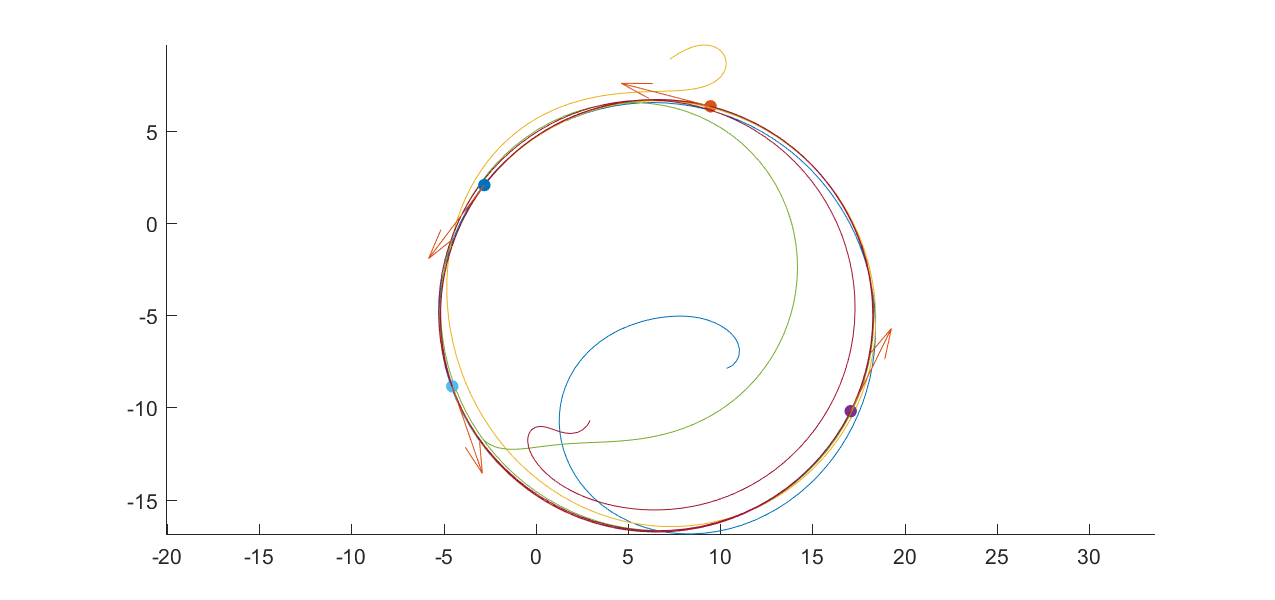
\includegraphics[width=\linewidth]{Attachments/Figure41.png}
	\caption{Circular formation with adaptive $\alpha$.}
	\label{fig:Adaptive}
\end{figure}

We now verify verify Observation 1 by simulation. The previous parameters are maintained and the radius control gain is changed to $\mu_r=.5$ and the reference radius is set to $r^*=10$. The formation now converges to a circle with a radius of 10 units as shown in Fig \ref{fig:RadiusConvergence}
\begin{figure}
	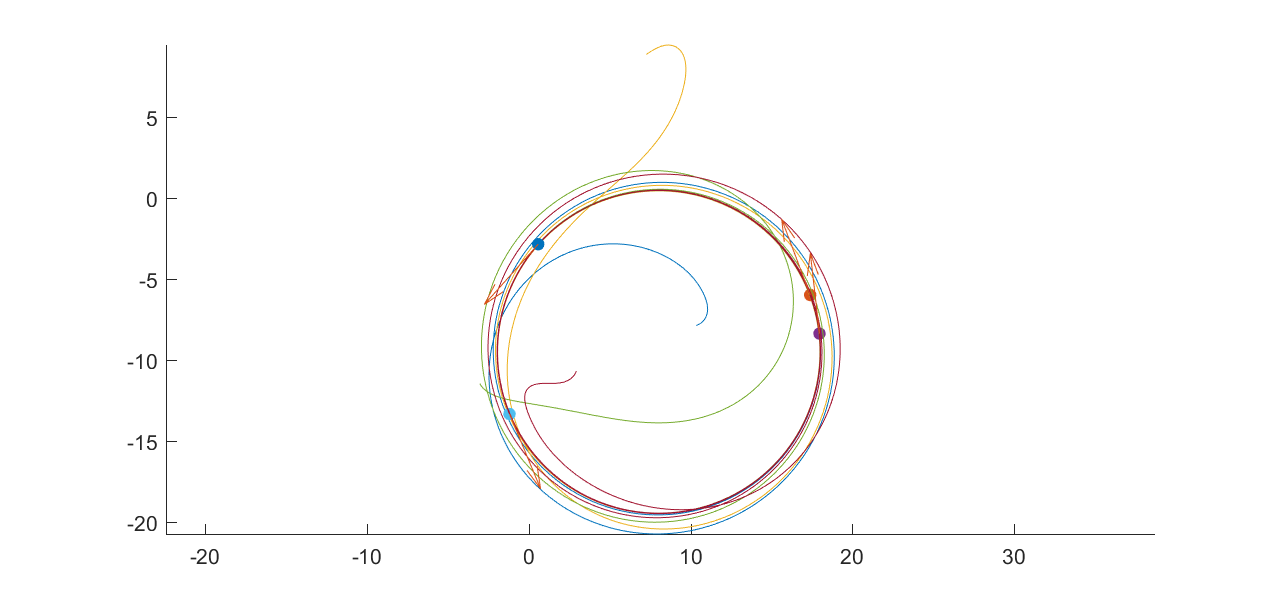
\includegraphics[width=\linewidth]{Attachments/Figure43.png}
	\caption{Circular formation with predetermined radius.}
	\label{fig:RadiusConvergence}
\end{figure}

For verifying Observation 1 the radius control gain is reverted to $\mu_r=0$. The equal spacing gain is chosen according to the guidelines provided, an order of magnitude smaller $\mu_s=.01$. The formation does not control radius but achieves an equally spaced formation as Fig  \ref{fig:EquallySpaced} shows.
\begin{figure}
	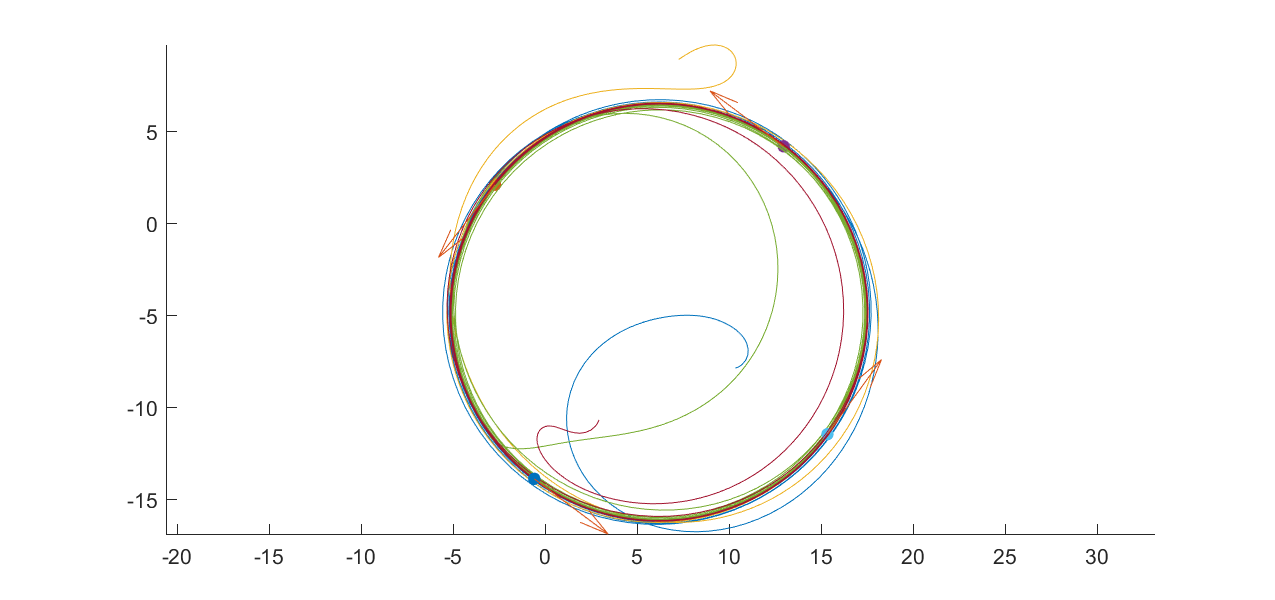
\includegraphics[width=\linewidth]{Attachments/Figure42.png}
	\caption{Equally spaced circular formation with adaptive $\alpha$.}
	\label{fig:EquallySpaced}
\end{figure}

Finally, all three control laws can be combined to achieve a circular formation with predetermined radius and equal spacing. A simulation is run with the previously used gains $\mu_c=.5,\mu_s=.01,\mu_r=.5$. The results for the complete algorithm are depicted in Fig \ref{fig:FormationConvergence}
\begin{figure}
	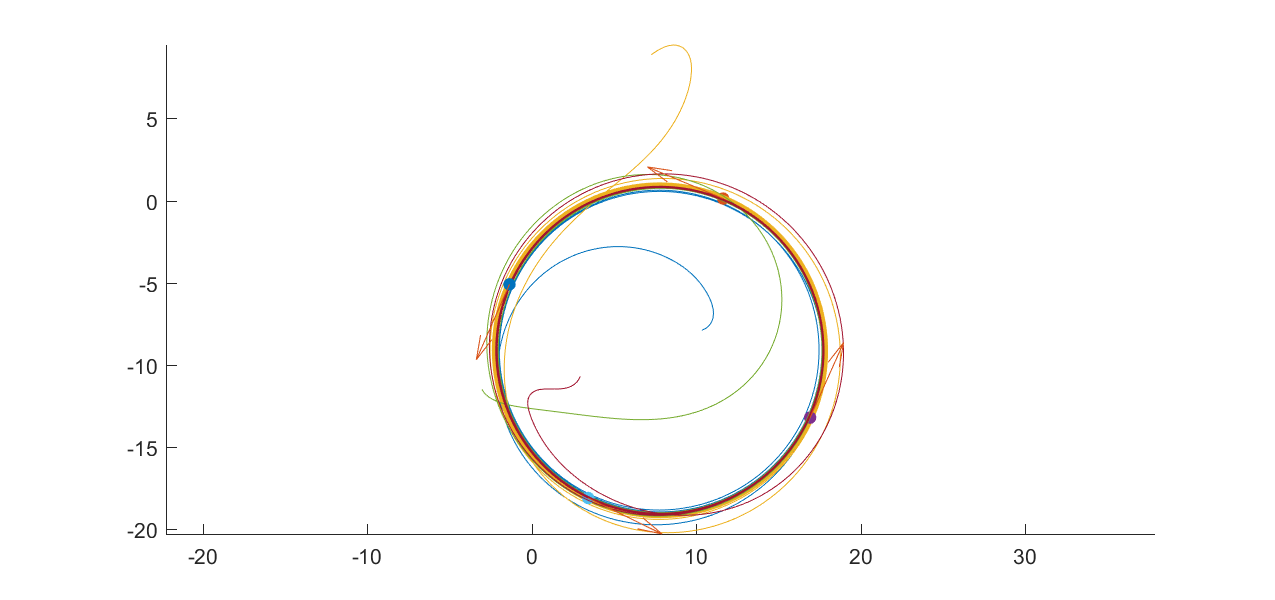
\includegraphics[width=\linewidth]{Attachments/Figure44.png}
	\caption{Equally spaced circular formation with predetermined radius.}
	\label{fig:FormationConvergence}
\end{figure}

Finally, an extra simulation is run to show the robustness of the formation to changes in the network. The following figure represents the way a formation that has already converged reacts to an agent joining the at the instant pictured in \ref{fig:Robustness}

\begin{figure}
	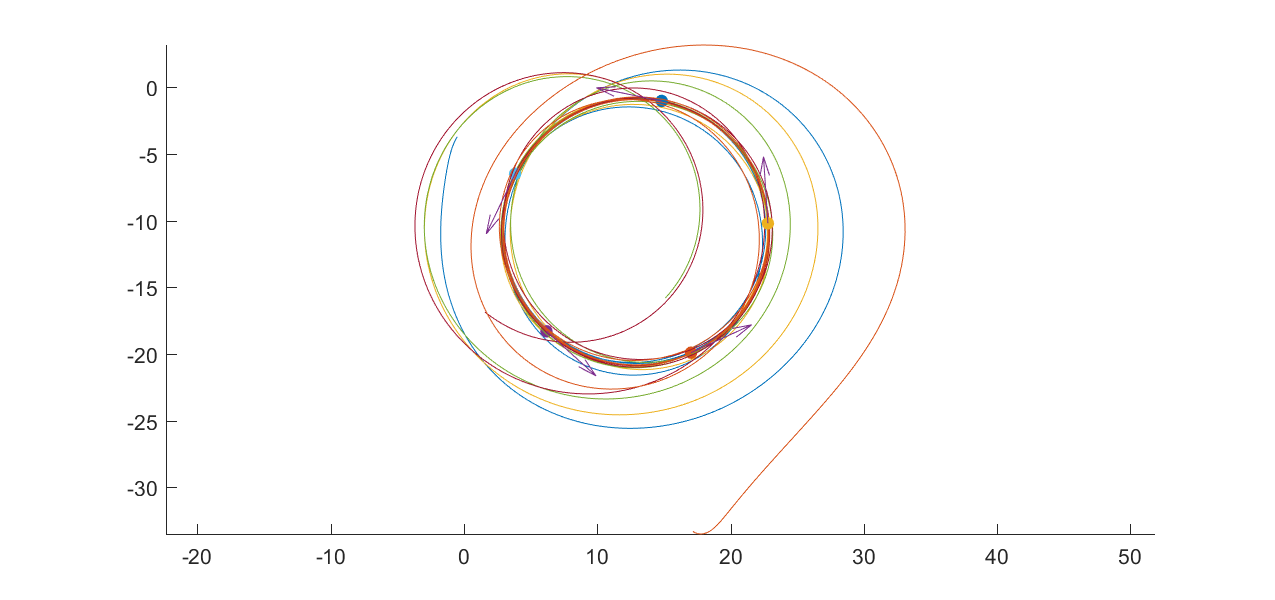
\includegraphics[width=\linewidth]{Attachments/Figure45.png}
	\caption{Robustness of the algorithm to changes in the network. The joining agent joins the formation from below.}
	\label{fig:Robustness}
\end{figure}
\section{Conclusion}

An adaptive control law is proposed that is able to make network converge to a circle using cyclic pursuit. The adaptive control law modifies the parameters used in cyclic pursuit in a distributed way in order to satisfy the global conditions for convergence. Furthermore, the adaptive control law uses only local measurements and does not need for any coordination between the agents. Beyond convergence to a circle, control laws for controlling the radius of the formation and achieving equal spacing are proposed. 

These three features: convergence to a circle, radius control and equal spacing (adding an extra measurement); allow for practical use of the algorithm for networks using only relative positioning. This is done by preserving the most relevant features of the original cyclic algorithm: global convergence and no need for communication between the agents. The proposed algorithm is not only feasible and implementable, it is also robust to changes in the network which is highly desirable for its integration into more complex systems.

Future work should address proving the convergence of the algorithm from a theoretical point of view. Only partial results for convergence are given in the Appendix. From a practical point of view, the integration of these findings with the strategy defined in \cite{pavone2007decentralized} for defining di-graphs in a decentralized way would allow to use the algorithm with no global coordination at all. Furthermore, it would be interesting to introduce control of the formation center when some agents have absolute positioning. Algorithms for circumnavigation such as those defined in \cite{deghat2010target} and \cite{deghat2014localization} could be of use for this purpose.

\begin{appendix}[Proof of convergence]
	We will use Lyapunov theory to prove the convergence of the formation. We will do that by showing that the achieved solution is an invariant and attractive set. This approach is different from those shown in other previous works since we use rely on an invariant set to which all cyclic pursuit formations converge to, this way we can prove global stability.

We start by describing the Cylic Pursuit manifold dynamics and then move on to proving the adaptive shape control law in (\ref{adaptiveLaw}) if the switching strategy is assumed to work perfectly. Only partials proofs for the circularization law are given.

\subsection{Assumptions and previous considerations}
Assumption 1 is critical since it states that the adaptive control laws are only effective in the cyclic pursuit manifold. 
\textbf{Assumption 2}. We will also consider that the gains are small enough so that the formation never leaves the cyclic pursuit formation manifold.

This assumption is somehow reciprocal to Assumption 1 in terms of convergence, but is better suited to out purpose here.

The closed loop dynamics under cyclic pursuit can be expressed in terms of the relative parameters $\kappa, \theta, \rho$ in a more compact way than absolute coordinates and introducing the agent $k$ as $k=\textrm{mod}(j+1,n)$ as shown in \cite{galloway2013symmetry}. 

\begin{align*}
  \dot{\kappa}_{ij} =& -v \mu \sin (\kappa_{ij} - \alpha_i) \\
  \dot{\theta}_{ji} =& -v \mu  \sin (\kappa_{ij} - \alpha_i)
  - \frac{v}{\rho_{jk}} (\sin \kappa_{jk} + \sin \theta_{kj}) \\
  &+ \frac{v}{\rho_{ij}} (\sin \kappa_{ij} + \sin \theta_{ji}) \\
  \dot{\rho}_{ij} =& -v (\cos \kappa_{ij} + \cos \theta_{ji})
\end{align*}

The equilibrium is given by an invariant set that satisfies $\kappa_{ij} = \alpha_i$. Furthermore, this set is shown  in \cite{galloway2013symmetry} to be attractive and Globally Asymptotically Stable (GAS). Also, if all $\alpha_i>0$ then it is guaranteed that $\dot{\theta}_{ji} \to 0$ also. Therefore the dynamics in the invariant manifold satisfy
\begin{align*}
  0 &= - \frac{v}{\rho_{jk}} (\sin \alpha_j + \sin \theta_{kj})
  + \frac{v}{\rho_{ij}} (\sin \alpha_i + \sin \theta_{ji}) \\
  \dot{\rho}_{ij} &= -v (\cos \alpha_i + \cos \theta_{ji})
\end{align*}

\subsection{Convergence to the circle}
Now we prove that the adaptive control law devised for circularizing the formation is stable when all other terms are 0, i.e. $\mu_r=\mu_s=0$. Then the formation converges to a circle.

While strictly satisfying Assumption 2 is impossible, if the shape control law is slow enough the approximation may be feasible. In that case, the invariant manifold behaves as
\begin{equation*}
  \dot{\alpha_i} = -\mu_1 \dot{\rho}_{ij} = v \mu_1 (\cos \alpha_i + \cos \theta_{ji})
\end{equation*}

The following Lyapunov function \cite{khalil1996nonlinear} is chosen
\begin{equation*}
  V = \sum_{i=1}^{n} V_i = \sum_{i=1}^{n} \frac{1}{2} \dot{\alpha_i}^2
\end{equation*}

This function is positive definite with a minimum $\dot{\alpha_i}=0$, this implies at the same time that $\dot{\rho}_{ij}=0$ or $\rho_{ij}$ constant. If we prove that $\dot{\alpha_i}$ is GAS since $V$ is radially unbounded then all the other hold by LaSalle's theorem. Operating on $V_i$ we get 
\begin{equation*}
  V_i = \frac{1}{2} \dot{\alpha_i}^2 = \frac{1}{2} v^2 \mu_1^2 (\cos \alpha_i + \cos \theta_{ji})^2
\end{equation*}

And now we compute $\dot{V}$
\begin{equation*}
  \dot{V}_i = \dot{\alpha_i} \ddot{\alpha_i}
\end{equation*}

So we have to find an expression for $\ddot{\alpha_i}$. Taking the time derivative on the expression we already have we get and realizing that 
\begin{gather*}
  \frac{d}{dt} \dot{\alpha_i} = v \mu_1  \frac{d}{dt} (\cos \alpha_i + \cos \theta_{ji}) = - v \mu_1 \sin \alpha_i \dot{\alpha_i} = \\
  - v^2 \mu_1^2   \sin \alpha_i (\cos \alpha_i + \cos \theta_{ji})
\end{gather*}

Here, we have assumed that the time derivative  $\dot{\theta}_{ij}$ is negligible since we are still arbitrarily close to the cyclic pursuit equilibrium manifold. Substituting
\begin{gather*}
\dot{V}_i = - v^3 \mu_1^3 \sin \alpha_i (\cos \alpha_i + \cos \theta_{ji})^2  v^2 \mu_1^2    (\cos \alpha_i + \cos \theta_{ji}) =\\
- v \mu_1 \sin \alpha_i V_i
\end{gather*}

Therefore the adaptive control law is Globally Exponentially Stable (GES) with rate of convergence $v \mu_1 \min (\sin \alpha_i)$, since we only use $\alpha_i \in [0,\pi]$. GES implies that the system is robust and then it will still converge if the system does not behave exactly as the equations of motion state. We stated beforehand that our adaptive shape control law would not completely satisfy Assumption 2. However, since the system is GES, the system will still be stable for small deviations.



\end{appendix}

\bibliographystyle{unsrt}
\bibliography{biblio}
\end{document}
